%!TEX program = xelatex
%%%%%%%%%%%%%%%%%%%%%%%这是导言部分的开始%%%%%%%%

%========= 导言部分声明文档的类型=================
\documentclass{article}

%=========导言部分可可以加载宏包=================
\usepackage{amsmath}                % 数学公式排版宏包
\usepackage{amssymb}                % 数学符号命令宏包
\usepackage{amsthm}                 % 数学定理宏包
\usepackage[UTF8]{ctex}             % 中文输入宏包
\usepackage[a4paper]{geometry}      % 页面设置宏包
\usepackage{setspace}               % 行间距宏包
\usepackage{graphicx}               % 图片宏包
\usepackage{listings}               % 代码宏包
\usepackage{color}					% 颜色宏包
\usepackage{xcolor}                 % 颜色处理宏包
\usepackage{float}                  % 浮动对象式样宏包
\usepackage{fontspec}
\usepackage{enumerate}				% 列举编号包

%=========页面设置==============================
\geometry{left=1cm,right=1cm,top=1cm,bottom=2cm}
\onehalfspacing
\setlength\parindent{0em}

%=========代码格式设置============================
\definecolor{dkgreen}{rgb}{0,0.6,0}
\definecolor{gray}{rgb}{0.5,0.5,0.5}
\definecolor{mauve}{rgb}{0.58,0,0.82}
% \setmonofont{Consolas}
\lstset{
	numbers = left, 	
	numberstyle = \color{gray}, 
	keywordstyle = \color{blue},
	commentstyle = \color{dkgreen}, 
	stringstyle = \color{mauve},
	basicstyle = \ttfamily,
	breaklines = true,
	frame = shadowbox, % 阴影效果
	rulesepcolor = \color{ red!20!green!20!blue!20} ,
	escapeinside = ``, % 英文分号中可写入中文
	xleftmargin = 2em,xrightmargin=2em, aboveskip=1em,
	framexleftmargin = 2em
} 

%=========导言部分可以定义标题信息===============
\title{组会报告}
\author{徐益}
\date{\today}
%%%%%%%%%%%%%%%%%%%%%%%这是导言部分的结束%%%%%%%%%

%%%%%%%%%%%%%%%%%%%%%%%这是正文部分的开始%%%%%%%%%
\begin{document}

%=========生成标题================================
\maketitle

%=========开始正文的输入==========================

%===========第一节=================
\section{工作内容} 
1. 对新接收数据解调译码;

2. 实现系统发送端5G编码调制链路。

%===========第一节=================
\section{解调译码结果}
\subsection{解调结果}
\begin{figure}[H]
	\centering
	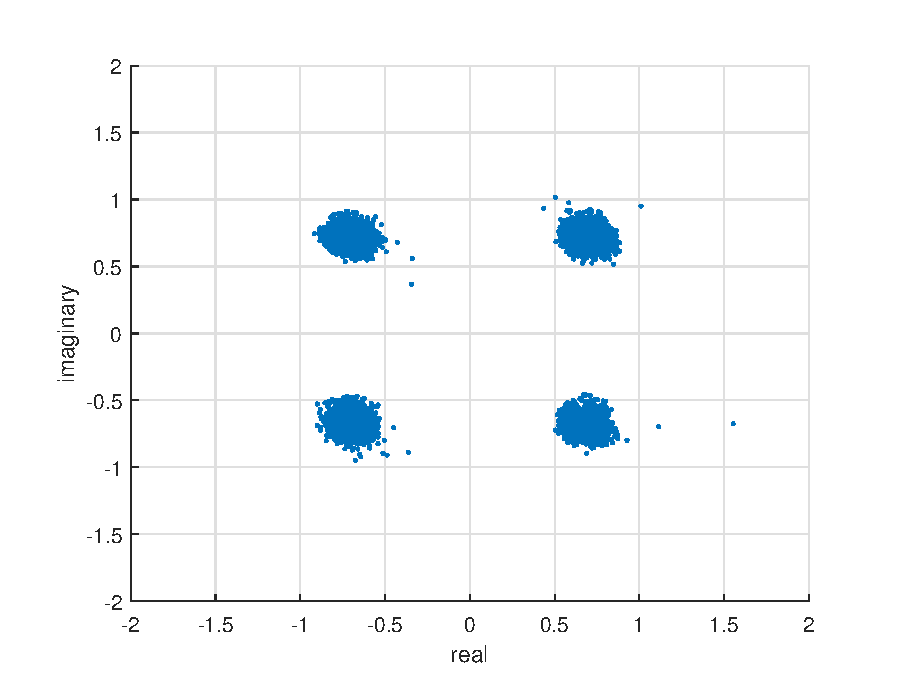
\includegraphics[width = .8\textwidth]{u2.eps}
	\caption{解调后星座图(QPSK)}
\end{figure}
\begin{figure}[H]
	\centering
	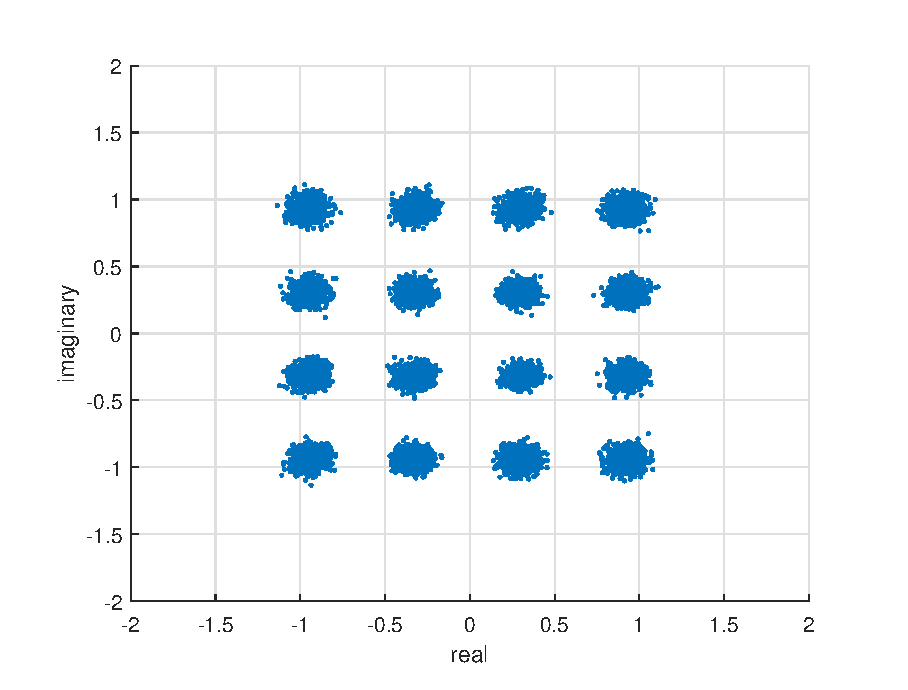
\includegraphics[width = .8\textwidth]{u3.eps}
	\caption{解调后星座图(16QAM)}
\end{figure}
\begin{figure}[H]
	\centering
	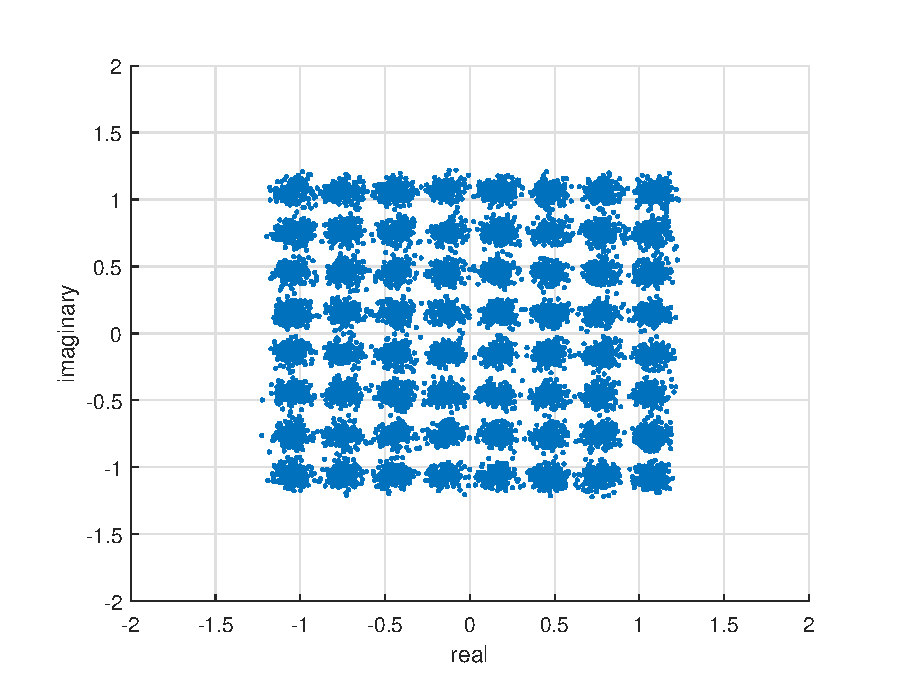
\includegraphics[width = .8\textwidth]{u4.eps}
	\caption{解调后星座图(64QAM)}
\end{figure}
\subsection{译码结果}
\begin{figure}[H]
	\centering
	\includegraphics[width = .8\textwidth]{res.png}
	\caption{译码结果}
\end{figure}

%===========第二节=================
\section{5GNR单线程编码调制链路的实现}
\subsection{改进点}
1. 系统的信息长度、CQI值、流数在每一次循环中均可变;

2. 改变用户个数与流数之间的关系;

3. 将主要处理过程封装为函数;

4. 增加SRS生成模块。

\subsection{Tx吞吐量测试}
\begin{table}[H]
	\caption{Tx各过程占比}
	\centering
	\begin{tabular}{|l|l|l|l|l|}% 通过添加 | 来表示是否需要绘制竖线
		\hline  % 在表格最上方绘制横线
		Process				& LTE		& 5GNR		\\
		\hline
		CRC Attach			& 8.80\%	& 9.65\%	\\
		\hline
		Code Blocks Segment	& 0.02\%	& 2.48\%	\\
		\hline
		Encode				& 21.89\%	& 23.31\%	\\
		\hline
		Rate Matching		& 44.63\%	& 42.39\%	\\
		\hline
		Map					& 12.23\%	& 16.25\%	\\
		\hline
		Pack				& 3.47\%	& 5.90\%	\\
		\hline  % 在表格最下方绘制横线
	\end{tabular}
\end{table}
Throuput\_Tx(LTE) = 103.32Mbps\\
Throuput\_Tx(5GNR) = 107.66Mbps

\subsection{Rx吞吐量测试}
\begin{table}[H]
	\caption{Rx各过程占比}
	\centering
	\begin{tabular}{|l|l|l|l|l|}% 通过添加 | 来表示是否需要绘制竖线
		\hline  % 在表格最上方绘制横线
		Process				& LTE		& 5GNR		\\
		\hline
		Channel Estimate	& 8.49\%	& 12.86\%	\\
		\hline
		Signal Detect		& 27.82\%	& 52.74\%	\\
		\hline
		Unpack				& -			& 1.52\%	\\
		\hline
		Link Adapt			& 9.86\%	& -			\\
		\hline
		Demap				& 3.51\%	& 10.19\%	\\
		\hline
		Rate De-matching	& 1.95\%	& 10.70\%	\\
		\hline
		Decode				& 41.69\%	& 11.67\%	\\
		\hline
		De-CBS				& -			& 0.30\%	\\
		\hline
		CRC Check			& 0.89\%	& 1.74\%	\\
		\hline  % 在表格最下方绘制横线
	\end{tabular}
\end{table}
Throuput\_Rx(LTE) = 9.17Mbps \\
Throuput\_Rx(5GNR) = 22.19Mbps
%===========第三节=================
% \section{根据PRACH测时延}
% \begin{figure}[H]
% 	\centering
% 	\includegraphics[width = \textwidth]{prach.png}
% 	\caption{时延测试结果}
% \end{figure}

%===========第四节=================
% \section{后续工作}
% 1. 实现当前SVN目录结构下基于LDPC的单线程编码调制链路;

%===========下周计划=================
\section{下阶段计划}
1. 完善单线程系统(修复Bug)

\end{document}
%%%%%%%%%%%%%%%%%%%%%%%这是正文部分的结束%%%%%%%%%%%%